%!TEX root = ../paper.tex

\subsection{Video} 
\label{label:video}

We experiment with YouTube and Skype applications to study the performance of video streaming and telephony, respectively. The set up and the QoE metrics used are described in \S\ref{sec:setup}. Similar to the Web experiments, we analyze application performance across 12 different CPU frequencies in one device and repeat the experiments over three smartphones. As before, we present the results from Nexus 4 and summarize the results from the other two phones.

%video applications are typically computationally intensive because of complex encoding and decoding techniques. At the same time, these applications are also network limited because of bandwidth constraints. In this section, we measure the impact of clock frequency and the second-order effect of network on YouTube and Skype QoE.





\begin{figure}[t]
  \centering
  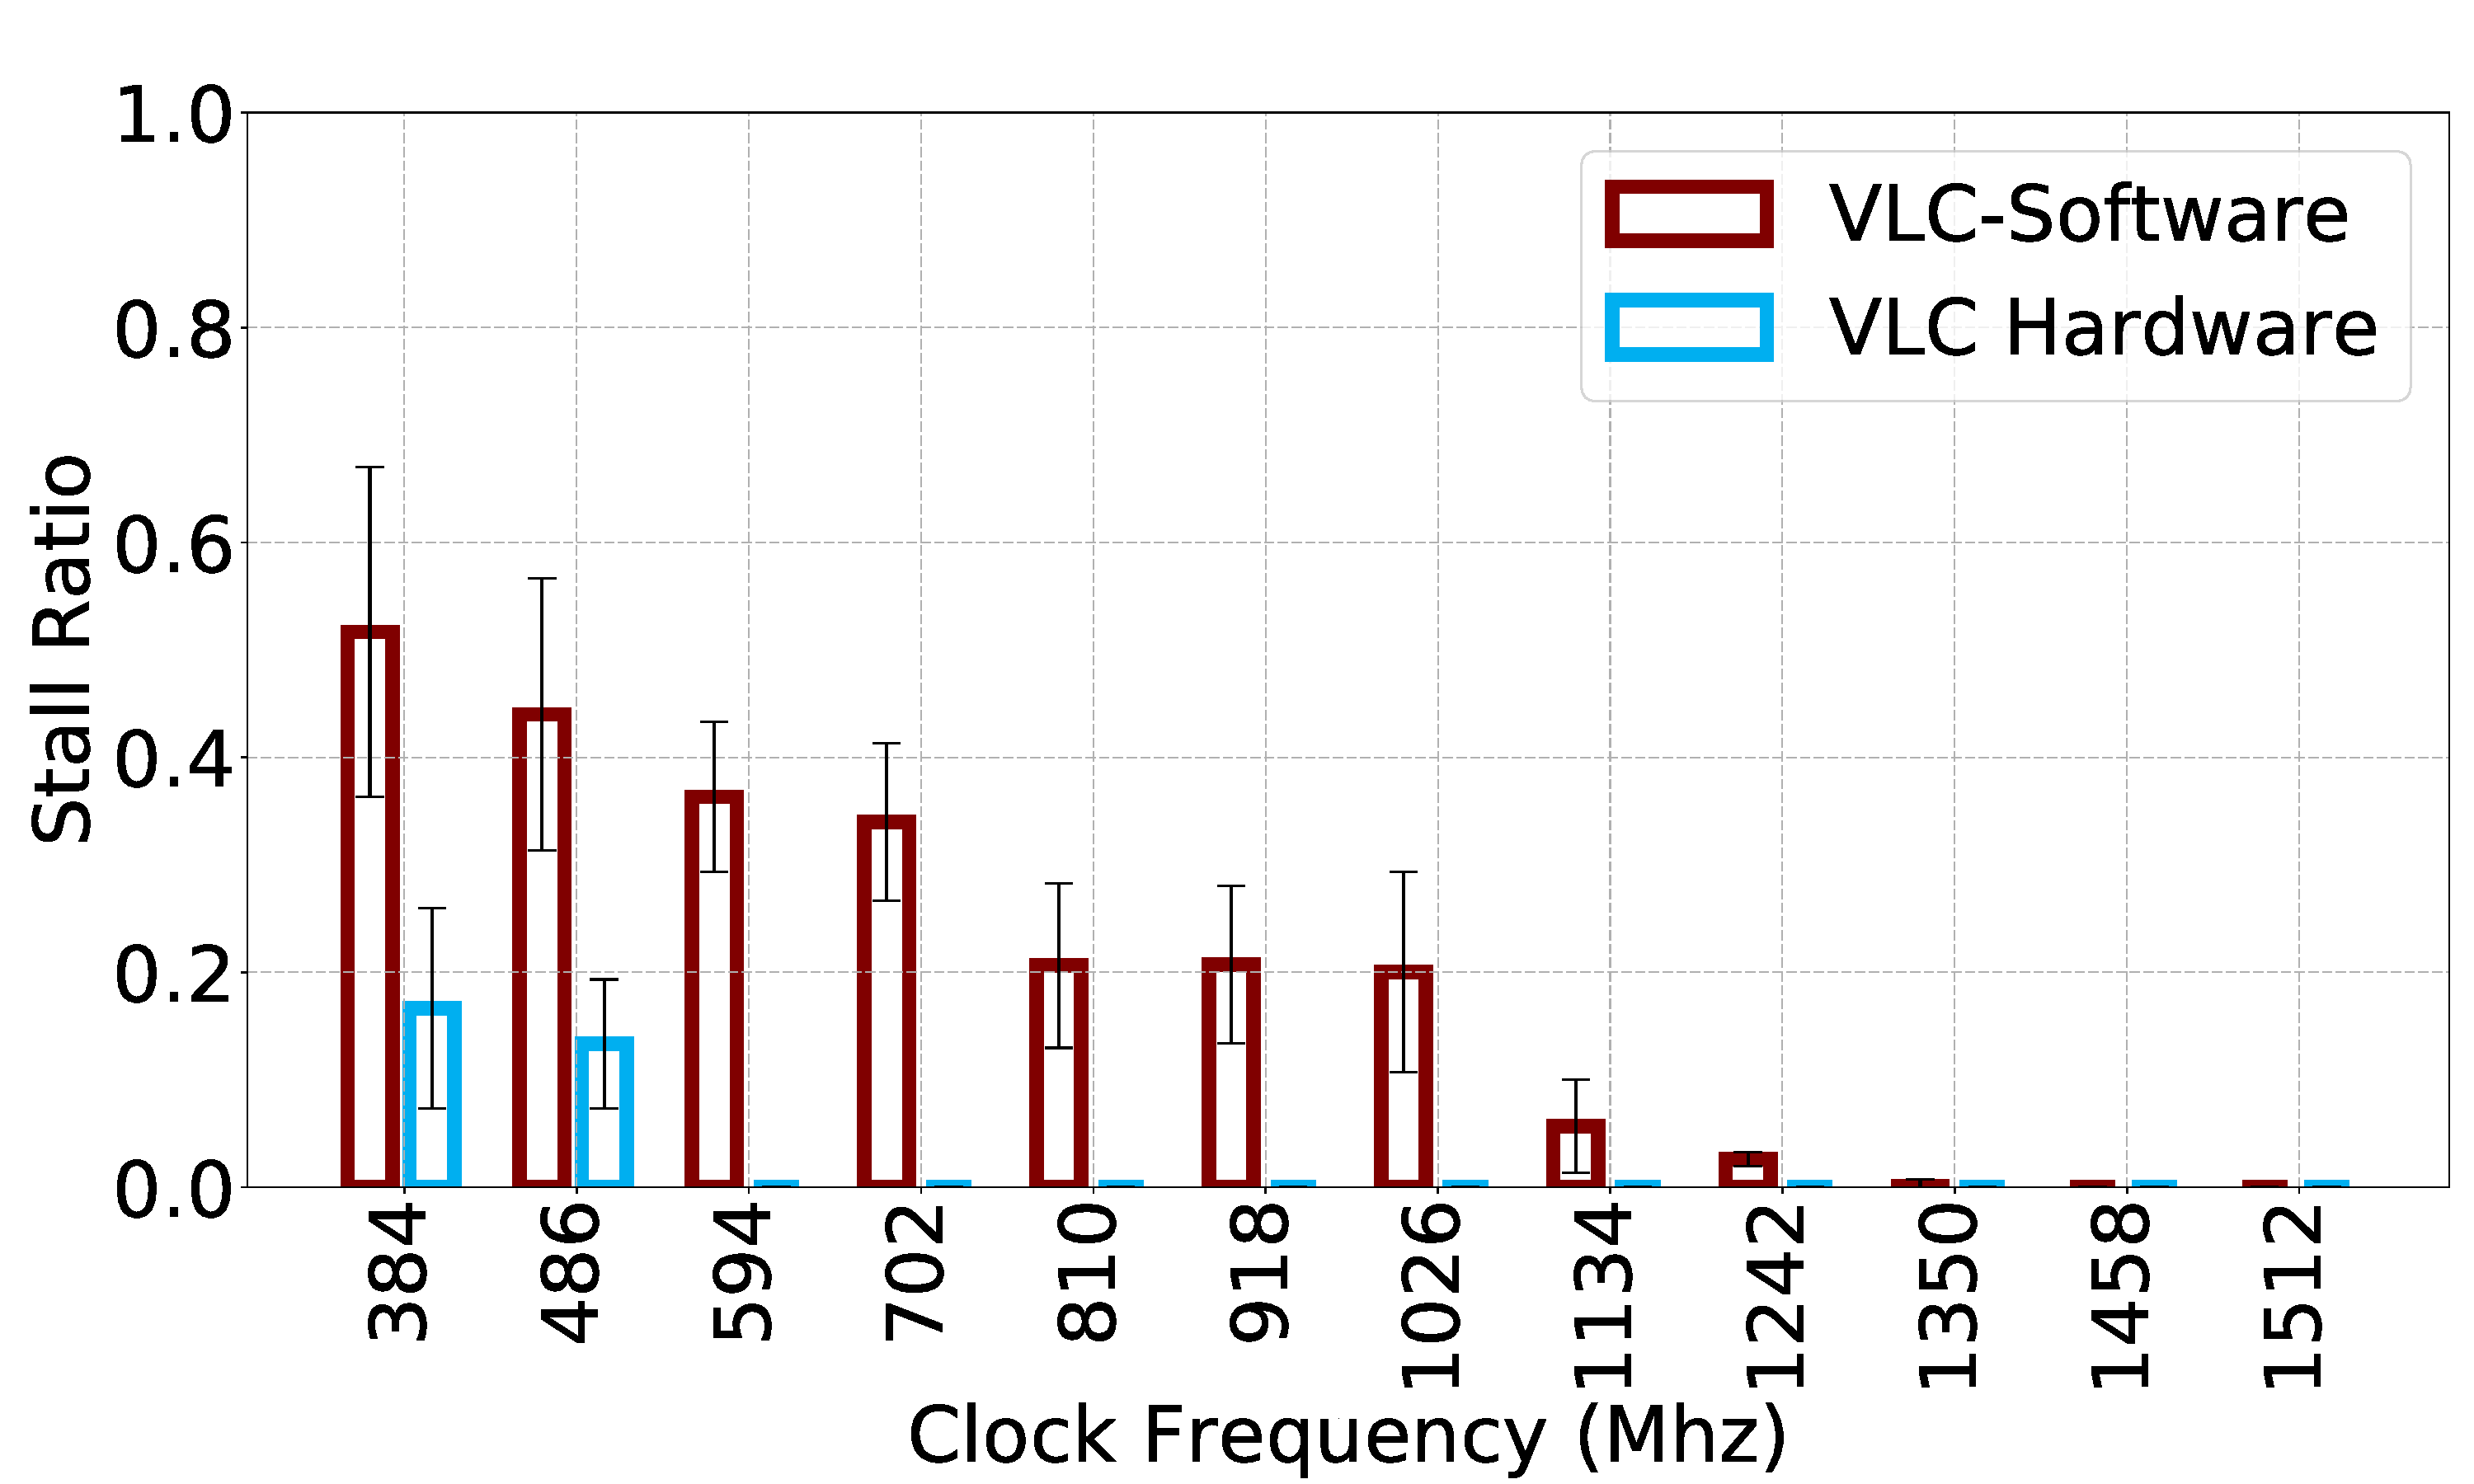
\includegraphics[width=0.8\linewidth]{sections/device-work/vlc-fps}
   \vspace{-0.1in}
     \caption{Isolating compute performance for video streaming by rendering videos locally via VLC player. When VLC is set to render in software, performance {\em is} affected by slow CPU. However, when  rendering is offloaded to hardware, CPU clock does not affect video rendering performance. All devices in our experiment (Table~\ref{tab:device_types}) offload rendering to a hardware decoder. }
   \vspace{-0.1in}
  \label{fig:vlc}
\end{figure}


\subsubsection{Video Streaming: YouTube}

Figure~\ref{fig:youtube}a shows the startup latency and stall ratio of YouTube for 12 different CPU clock frequencies on Nexus 4. 
The startup latency increases from 1.2 to 3.5 seconds as the clock speed decreases, however 
there is no impact on the stall ratio. Even though the bitrate adaptation algorithm is turned on during our experiments, we do not see any change to the video resolution during the experiment.

This trend is similar to the one observed in Figure~\ref{fig:motivation}b across low-end and high-end phones. Experiments on Intex Amaze+ and Google Pixel 2 show quantitively similar trends (not shown here).


%Our goal is to  (a) study the effect of CPU speeds on the network and compute components of video streaming, and (b) investigate why CPU speeds have no effect on the stall ratio, despite streaming being a compute-intensive application.
% clock to low clock.
%We note that the fall in start-up latency is not gradual, but falls much faster at lower frequencies than at higher frequencies. 
%Interesting, the stall ratio has zero effect even under lower clock.
%This is a counter-intuitive result, since we had seen that even network throughput gets significantly slowed down at lower frequencies. 
%This descrepancy is due to two reasons: First, the computation effect of clock is removed because of hardware accelerated video decoding. Second, the impact of clock on network also not affecting YouTube streaming because of prefetch capability. 
%Although we see a significant impact of clock in the begining of video playback, we do not observe any quality degration i.e the resolution of video and no stalls ratio even under lower clock. 
%We first explain the overall impact of clock on YouTube video QoE, then we isolate the impact of clock on network and compute. We use the similar set-up used for YouTube in Section \ref{sec:motivation}

%YouTube player starts a video with an initial wait time to prefetch some future portion of video. 
%After the start-up time, it makes sure to prefetch further video content for certain (120seconds) duration. 

\noindent \textbf{Network:} During video streaming, video content is downloaded from the network and then processed by the video decoder. Unlike the Web, the network and compute operations are not inter-leaved, making it easier to separate the two. To isolate the effect of network on video performance, we measure application QoE before video decoding. We first estimate the {\em time-to-first-frame}, as the time it takes to download video content before the first frame is displayed. Our experiments show that the difference in time-to-first-frame between slow and fast CPU can explain the startup latency performance in Figure~\ref{fig:youtube}a. The time-to-first-frame increases when the CPU speed is low because it takes longer to process the TCP packets, affecting the startup latency (results omitted for brevity). In fact, the start up latency is not affected by the compute operations at all.

In practice, the stall ratio is a more important QoE metric, since the startup latency is only a one-time effect. We first look at why the stall ratio is not affected under slow CPU conditions, even though network throughput drops when the CPU is slow. YouTube and other video streaming services~\cite{netflix,hbogo} prefetch video content; YouTube prefetches 120 seconds worth of content. The Read Ahead Convergence (RAC) time is the time required for YouTube to fetch  120 seconds worth of content. 

Figure \ref{fig:youtube}b shows the RAC time across different CPU speeds.  There is a difference of 25 seconds in RAC time between the slow and fast CPU clock. However, even under slow clock, the RAC time to fill the buffer is well under 120 seconds required to play the video. Therefore, the increase in RAC time does not introduce any stalls, resulting in no effect on the stall ratio.  %\mallesh{It is important to note here that YouTube server is not detecting such low network condition at the client and not adapting the bitrate i.e., we found the same video resolution even under slower clock.}




% the default read-ahead buffer. YouTube, as well as other video streaming services~\cite{netflix, hbogo}, maintain a fixed buffer worth of video data, so that users do not experience stalls. In the case of YouTube, this buffer contains 120 seconds worth of video content. % \todo{I dont understand this 120 second time}
%The RAC time is the time required for the YouTube to reach the default read-ahead time. That is, YouTube maintains a fixed 120seconds read-ahead time for the user so that the user does not experience any stalls during the playback. 
%Ideally, the RAC time takes 10 to 12 seconds to fill the read-ahead buffer. 

\begin{figure*}
\begin{minipage}[t]{.33\textwidth}
   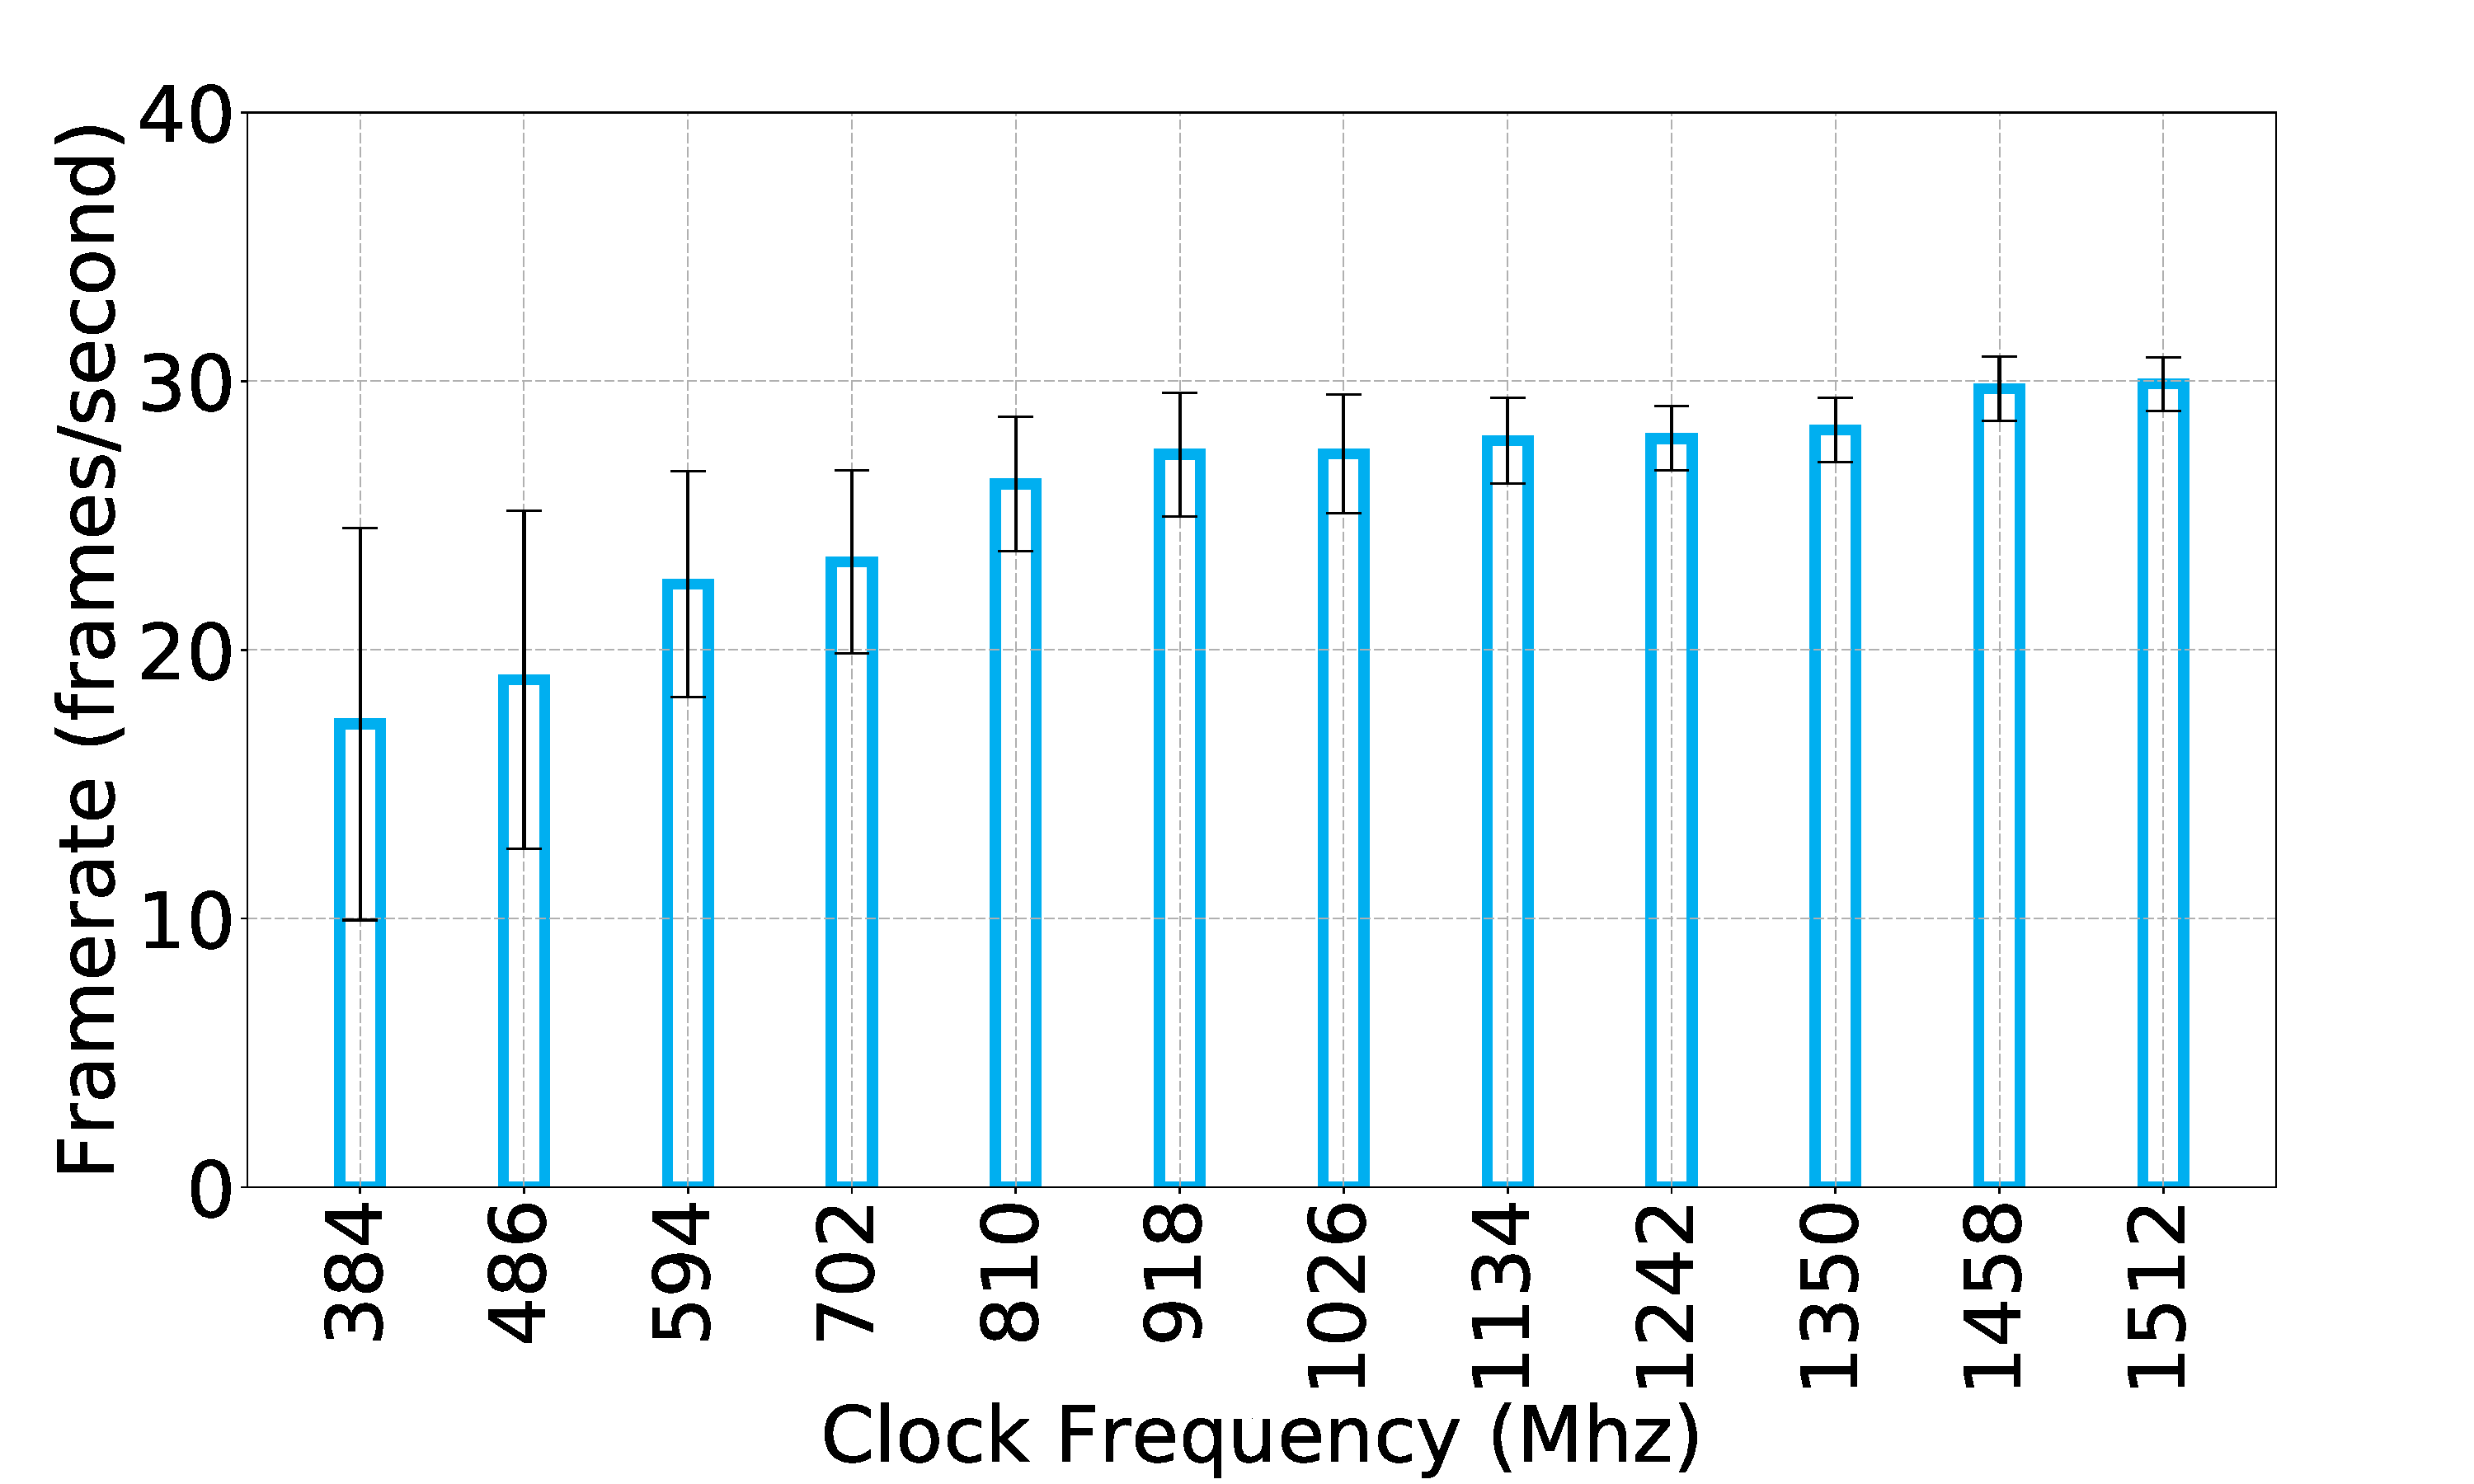
\includegraphics[width=\linewidth]{sections/device-work/skype-fps.pdf}
   \caption{Skype QoE: The frame rate decreases by 33\% when the CPU clock speed decreases.} 
   \vspace{-0.2in}
   \label{fig:skype-framerate}
\end{minipage}
\hspace{0.1in}
\begin{minipage}[t]{.33\textwidth}
   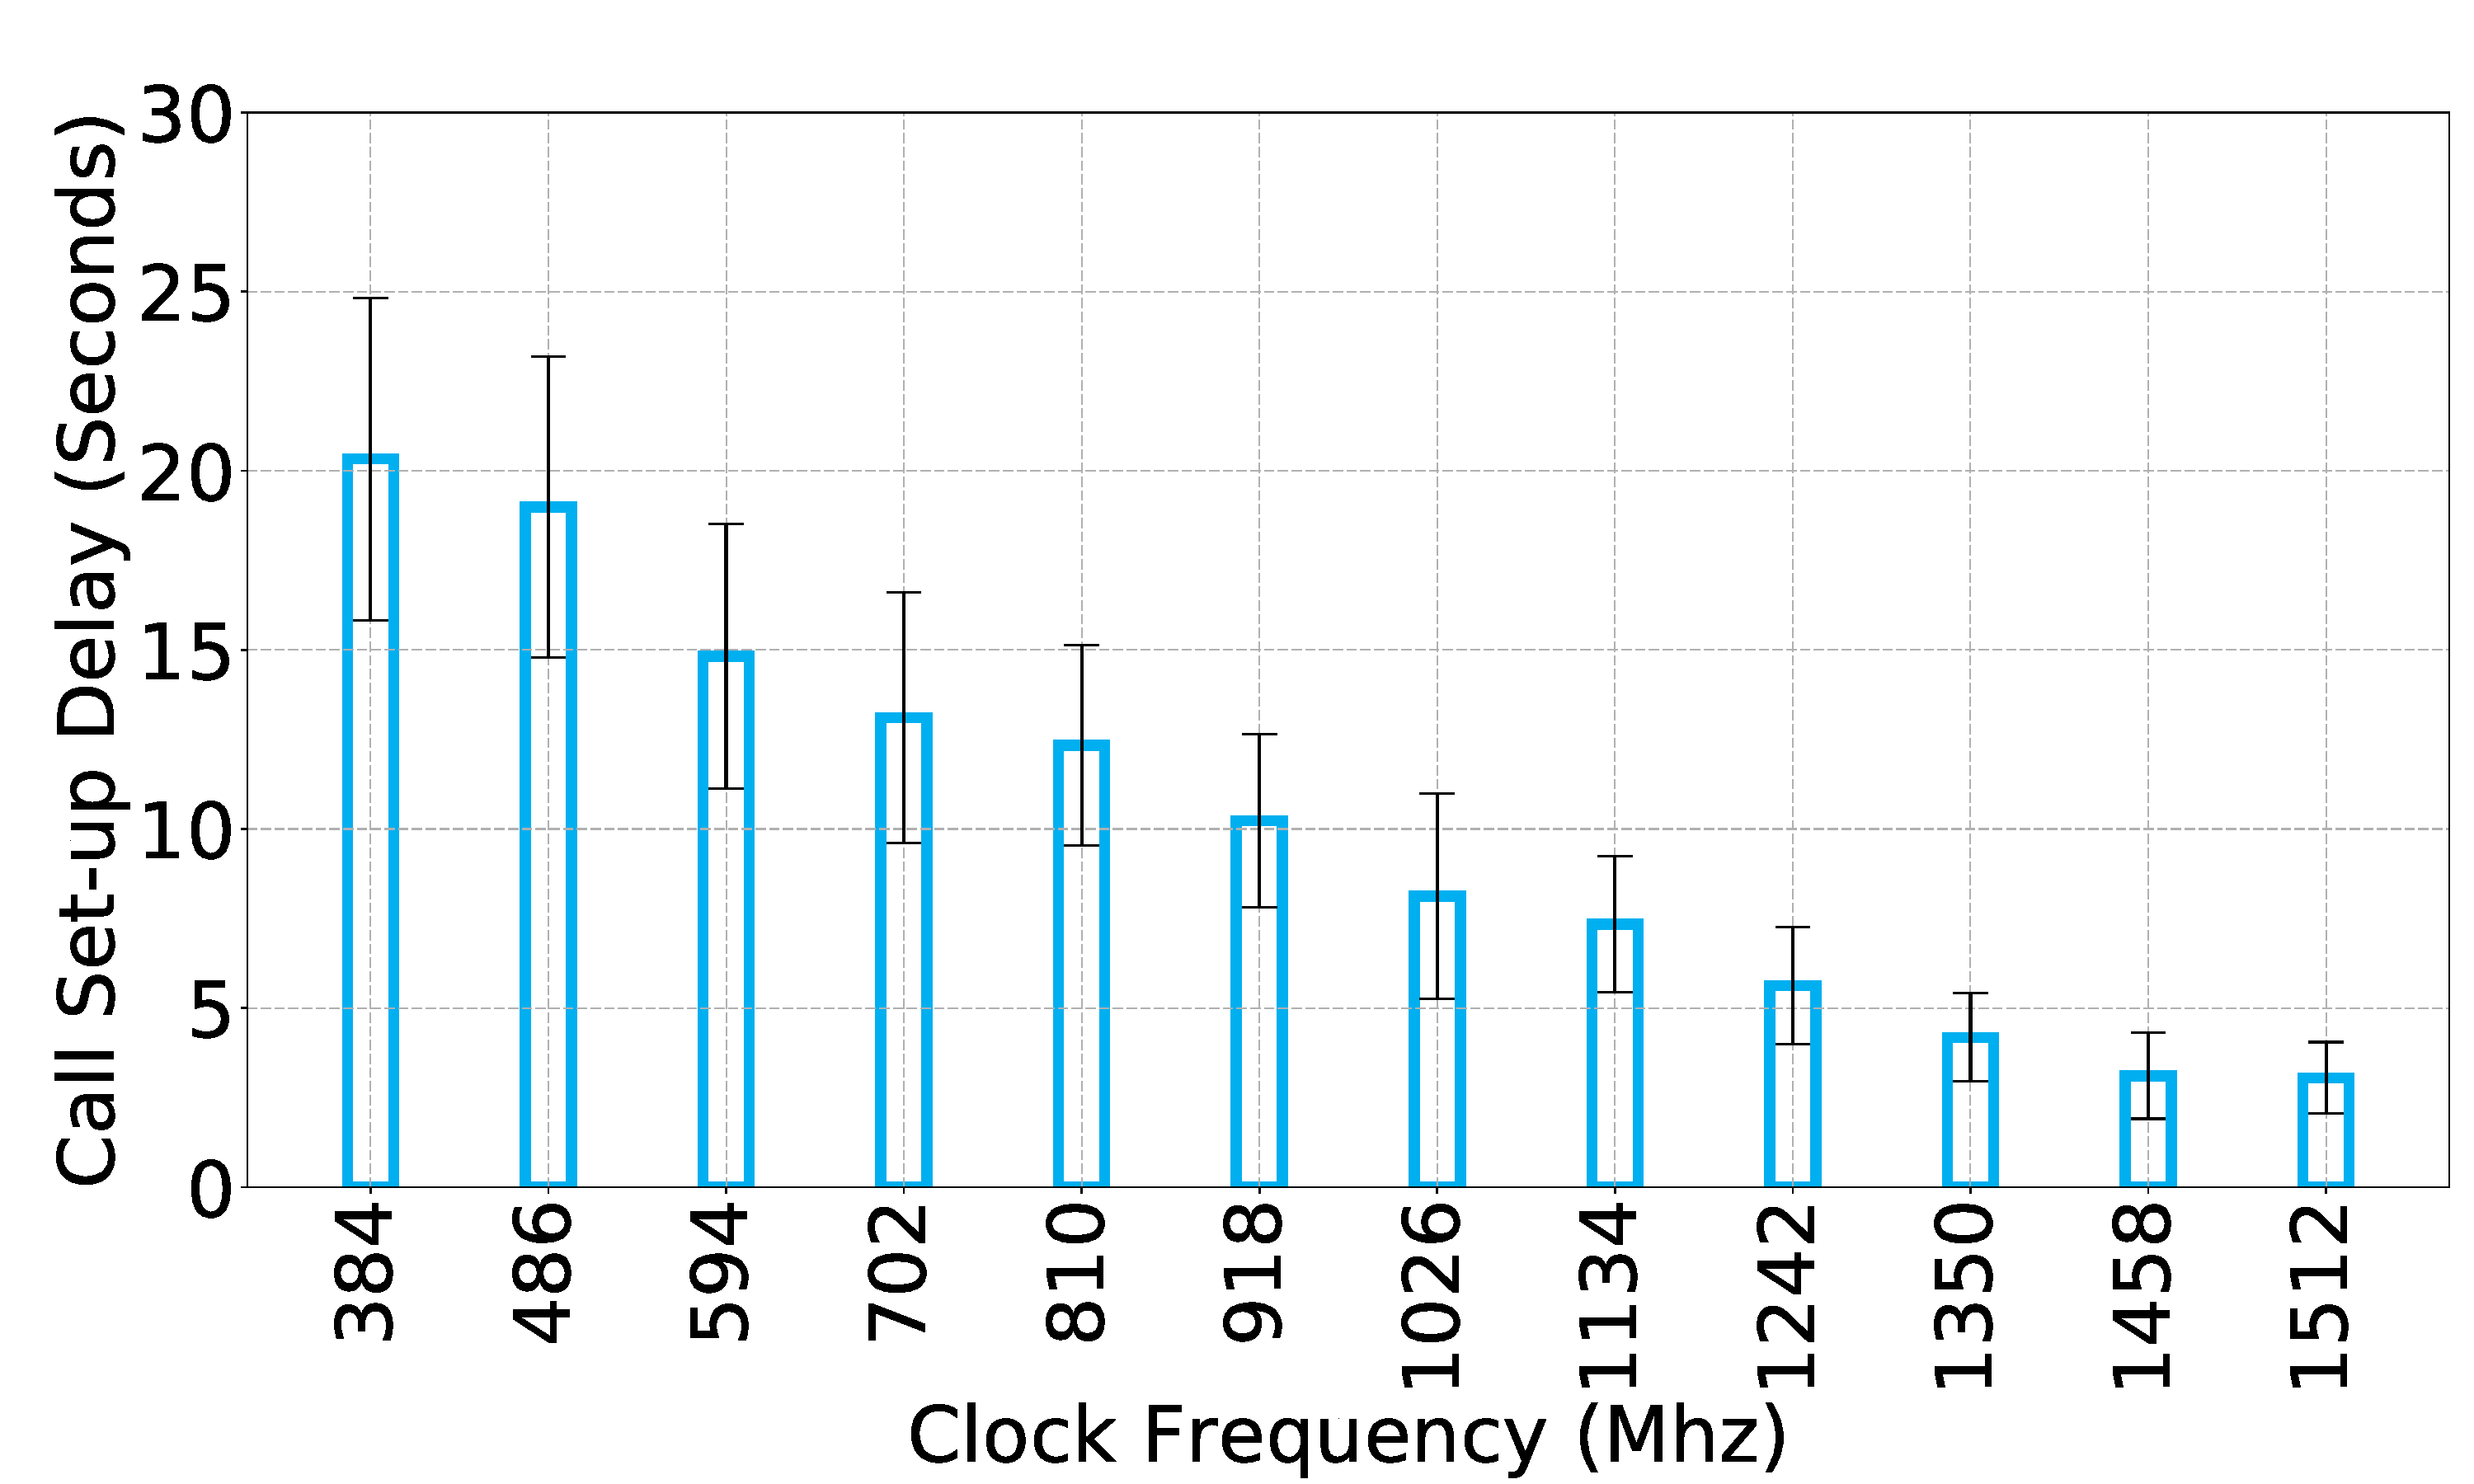
\includegraphics[width=\linewidth]{sections/device-work/skype-call-setup.pdf}
   \caption{Effect of CPU speeds on the network-centric metric, call set-up delay.} 
   \vspace{-0.2in}
   \label{fig:skype-call}
\end{minipage}
\hspace{0.1in}
\begin{minipage}[t]{.33\textwidth}
   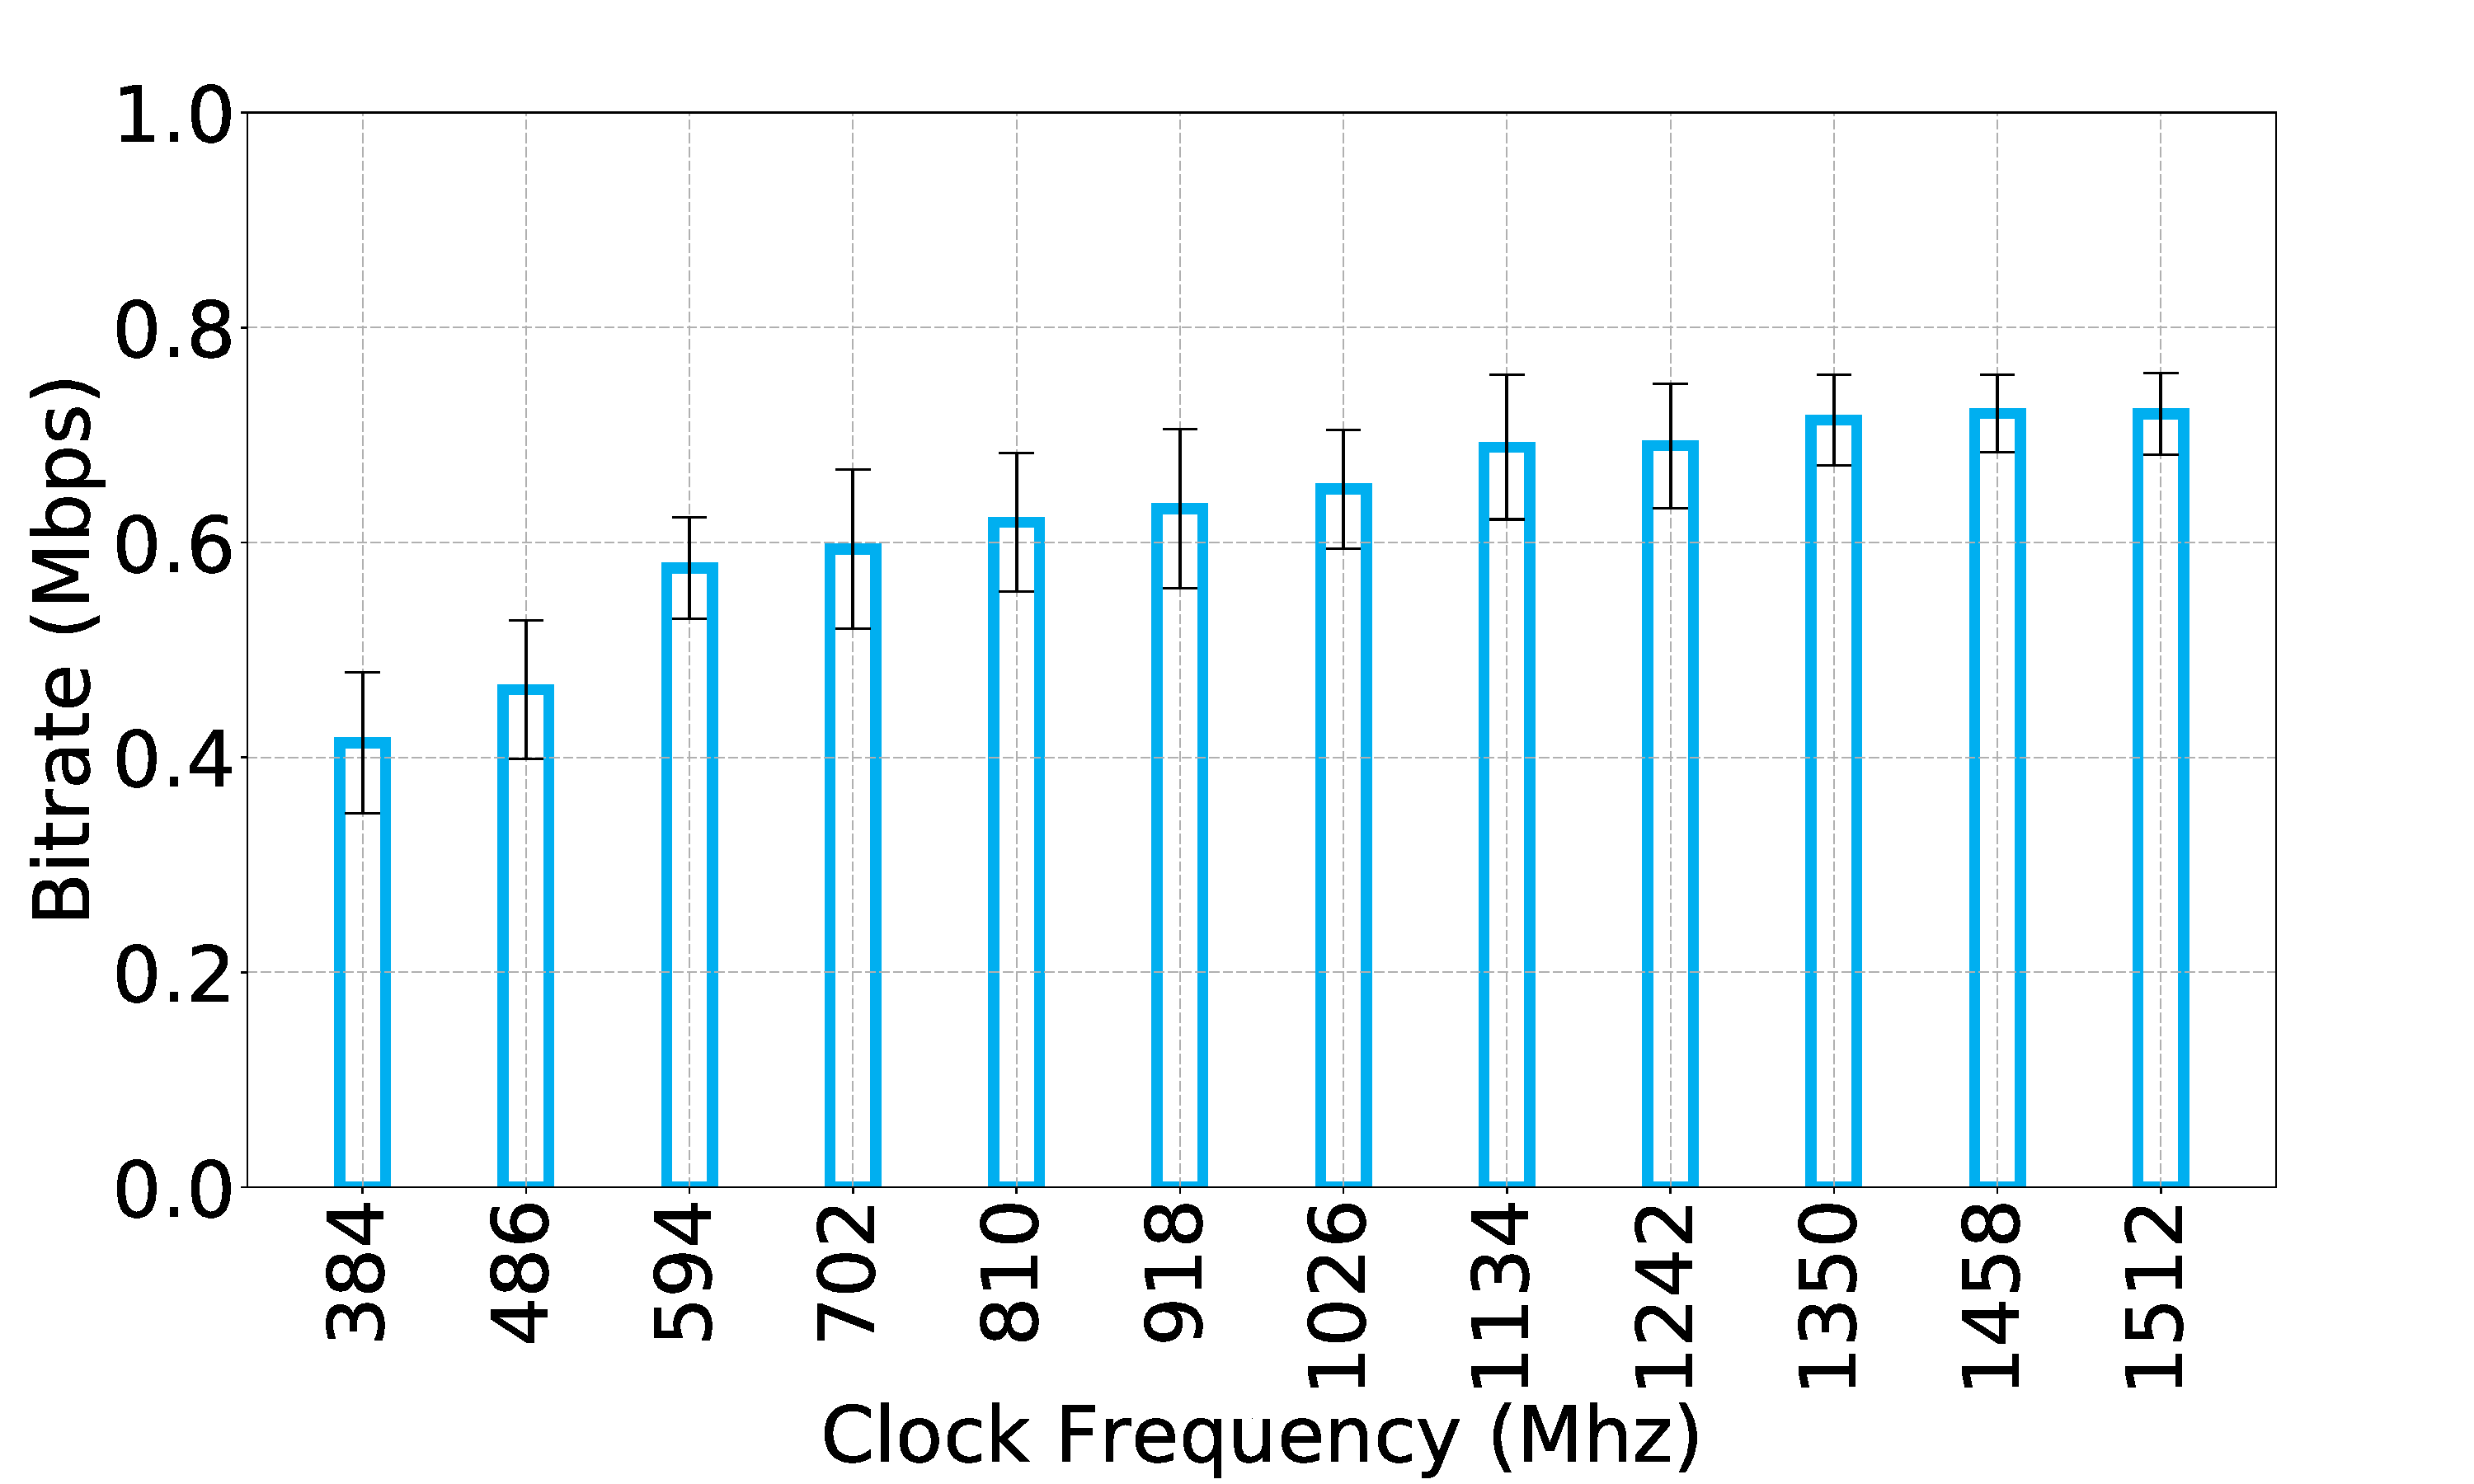
\includegraphics[width=\linewidth]{sections/device-work/skype-bitrate.pdf}
   \caption{Effect of CPU speeds on the network-centric metric, bitrate.} 
   \vspace{-0.2in}
   \label{fig:skype-bitrate}
   \end{minipage}
\end{figure*}

\noindent \textbf{Compute:} Isolating the effect of compute for YouTube is harder because YouTube is a closed application, making it hard to modify the application. Instead, we conduct a set of experiments on VLC player~\cite{andriodvlc}, an open-source streaming application, and change the VLC player to use either software or hardware rendering/decoding. Our goal is to understand why streaming applications do not take a hit under slow CPU, even though video streaming is a compute-intensive application.  

Hardware rendering involves offloading rendering and video decoding to hardware, which may either be the GPU or an in-built hardware accelerator. Software rendering refers to when the rendering and decoding is done in software.
We cross-compile the Android VLC open source~\cite{andriodvlc} using Android SDK tool chain~\cite{andriodsdk}. 

 %We play a locally stored video using the VLC player and alternate between software and hardware rendering/decoding.  % All phones, including the lower-end phones in our experiment, are equipped with the hardware accelerator. %. The same video described in Section \ref{sec:motivation} is used in our experiment. We tap the source code to extract Framerate during the playback. Typically, if the frames are not decoded within the display timestamp, the player drops such frames and the video gets frozen. This happens because of the slower processing of video decoding. 

Figure \ref{fig:vlc} shows that when decoding and rendering is performed in software, the stall ratio increases to 0.5 under slow CPU. In contrast, under fast CPU, the video experiences nearly no stalls. However, when decoding and rendering is offloaded to hardware, CPU speed only has a small effect on stall ratio when using the VLC player. Our earlier experiment shows that over YouTube, the effect of CPU speeds on stall ratio is in fact zero. 

We verify (using Android logs)  that YouTube indeed offloads video decoding to an in-built hardware, different from the GPU, and does not perform rendering in software. %The key takeway is that if video processing is offloaded to hardware, applications do not experience stalls even with under slow CPU. This is in fact what is happening in our experiments. 
 In fact, the hardware video decoder is available across all devices we tested, including the low-end Intex Amaze+ device. As a result, the stall ratio is not affected by CPU speeds.

 %shows the impact of clock under two different settings -- with CPU and GPU video decoding respectively.
%With CPU decoding, the Framerate goes to as low as 15Fps under low clock. However, after 1242Mhz clock, we do not see any effect of clock as the CPU is able satisfy 30Fps requirement.
%However, if the GPU is enabled, we observe a consistent 30Fps util 594Mhz clock and a 5Fps reduction under very lower clocks. 
%Thus, the presence of the GPU improves the QoE of video rendering on smartphones even when the clock frequencies are low.



\subsubsection{Video Telephony: Skype}

The key difference between streaming and telephony is that telephony is interactive. This means that unlike streaming,  video frames cannot be prefetched by the application. The performance of telephony is measured in terms of frame rate %and the call set-up time. The call set up time is the time between when call is initiated by one client and answered by another client. 
and the measurement set-up is described in \S\ref{sec:setup}.

Figure~\ref{fig:skype-framerate} shows the effect of clock frequency on frame rate during the Skype video call. 
The frame rate drops to 17 frames-per-second (fps) at slow CPU speeds from 30 fps at high CPU speeds. 
%% Aruna: I am removing this since its quite tedeous.
%Interestingly, the standard deviation in frame rate at 384 Mhz and 486 Mhz is more that 8 fps, as shown by the error bars.
%This is because the adaptive bitrate algorithm~\cite{sodagar2011mpeg} used by Skype changes the video resolution. Typically, the bitrate algorithm reacts to changes in the the network condition. However, in our experiments, the network condition does not change.  In effect, the Skype client perceives the network performance to be poor because of the increase in packet processing delays at slow CPU frequencies. The result is that the client often requests low resolution videos under slower clocks causing the fluctuations in the frame rate.

%We note that the bitrate increases very slowly after reaching $600Kbps$ at a clock frequency of $594Mhz$. 
%The bitrate is also very low in case of lower clock because of two reasons: One is due slower packet processing (see \ref{sec:throughput}) and second, because of adaptive bitrate algorithm at the client2, it is receiving low resolution video. That is, Skype server is treating low clock as poor network at client1 and informing the client2 of video call. This makes client2 to send low resolution video. This is happening mostly under very low clock i.e 384Mhz clock. This is because of huge variance in throughput under lower clocks. The change in bitrate follows the same trend as the change in network throughput we saw in Section \ref{label:throughput}. 

%The framerate shows different characteristic than bitrate. The variance in framerate is very high under low clock. This is due to adaptive bitrate algorithm: we see increased framerate when there is lower resolution and decreased framerate under high resolution. 

\noindent \textbf{Network:} 
To see the isolated effect of clock on network, we measure two network-centric metrics: call set-up delay and bitrate during the Skype call. 
The call set up delay is the time between when the mobile client initiated the call and when the server accepted the call. We measure the call set up delay using the our screen recordings, as described in \S\ref{sec:motivation}. The bit rate is the number bits received per second. The bit rate is different from the frame rate since it does not include rendering. Both bit rate and call set-up delay only depend on the network performance.

%\footnote{The call start-up delay can be more if the other client does not respond soon. But, note that in our set-up the other client automatically responds as soon as it receives the call, so there is no effect from other client.} is the time it took for client1 to receive the call acceptance from client2. 


Figure \ref{fig:skype-call} shows the impact of CPU speeds on the call set-up delay.
We observe a 18 second increase in call start-up delay when the CPU clock reduces from 1512 MHz to 384 MHz. This effect is due to the increase in network packet processing caused by slow CPU speeds, since the external network condition remains the same. Figure \ref{fig:skype-bitrate} shows the impact of clock on bitrate. 
Again, we see that the bitrate decreases from 700 to 400 Kbps at slow CPU clock speeds. The key takeaway is that video telephony is significantly affected by slower CPU speeds because of the network processing delays. This is different from video streaming, where the effect of the network processing delays is masked by prefetching.


%Note that the call start-up delay has no compute component and is a network intensive and hence impacted by throughtput drop (\S\ref{label:throughput}) with with respect to clock.





 %Note the stadard deviation is not as high as in the case of framerate. This is again due two reasons: First, as the clock rate reduces, we find that the adaptive bitrate algorithm reduces the resolution of the video, significantly reducing bitrate. The second reason is because of decrease in throughput.

\noindent \textbf{Compute:} In terms of compute, there is little difference between streaming and telephony; both involve processing and rendering video frames on the screen. Similar to YouTube, Skype offloads rendering to the hardware decoder. As a result, changing the CPU clock frequency has little effect on telephony from the compute standpoint.
